\begin{frame}{Function Approximation}

    Why Function Approximation?

    \begin{itemize}
        \item large state spaces
        \item slow learning
        \item need for generalization
    \end{itemize}

\end{frame}

\begin{frame}{Naive Function Approximation}
    \begin{equation*}
    Q(s,a,\theta ) \approx Q(s,a)
\end{equation*}

\begin{equation*}
    \mathcal{L}(\theta )=\E \left [\Bigg( r+\gamma\max_{a'} Q(s',a',\theta )-Q(s,a,\theta )\Bigg)^2\right] 
\end{equation*}

\begin{equation*}
    \pfrac{\mathcal{L}(\theta )}{\theta }=\E \left [\Bigg( r+\gamma\max_{a'} Q(s',a',\theta )-Q(s,a,\theta )\Bigg)\pfrac{Q(s,a,\theta )}{\theta }\right] 
\end{equation*}


\end{frame}

\begin{frame}{Deadly Triad}

   \metroset{block=fill} 
    \begin{alertblock}{Deadly Triad}
        \begin{itemize}
        \item function approximation
        \item off policy learning
        \item bootstrapping
        \end{itemize}
	\end{alertblock}
      

\end{frame}

\begin{frame}{DQN}

   \metroset{block=fill} 
    \begin{alertblock}{Deadly Triad}
        \begin{itemize}
        \item function approximation
        \item off policy learning
        \item bootstrapping
        \end{itemize}
	\end{alertblock}
      

\end{frame}

\begin{frame}{atari arcade games}
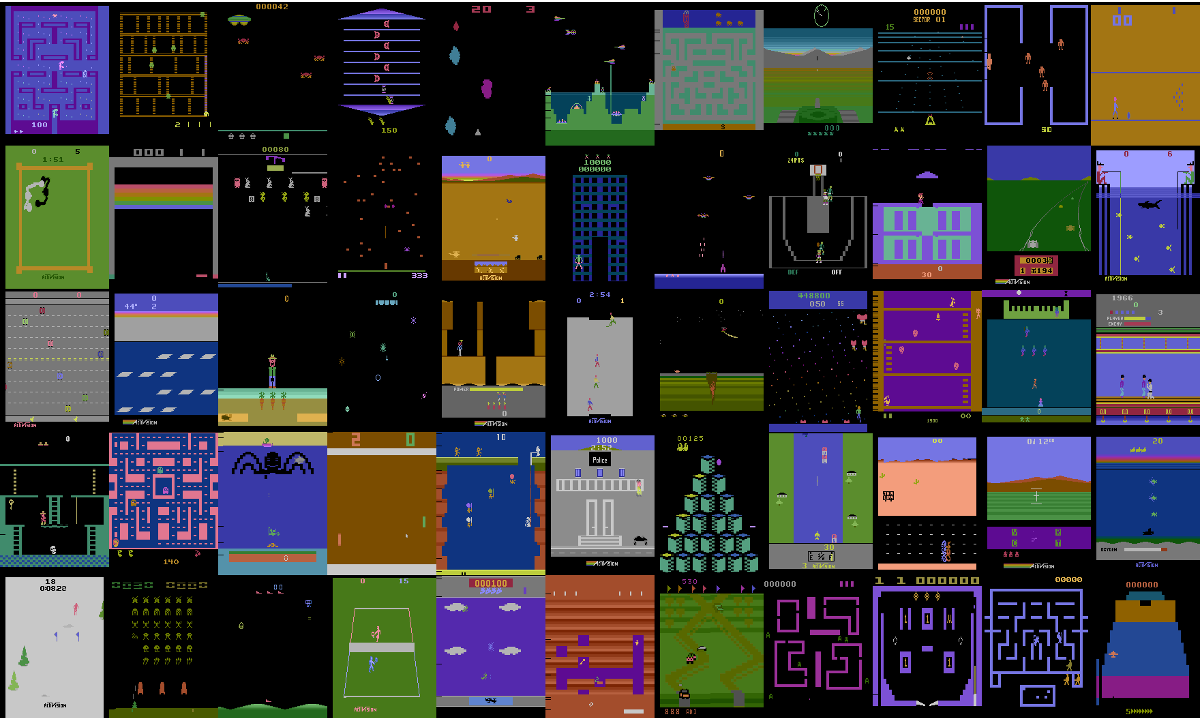
\includegraphics[height=\textheight,width=\textwidth,keepaspectratio]{atarigames}
\end{frame}


\begin{frame}{DQN}
   \textbf{\textsc{Human-level control through deep reinforcement learning}}\footnote{\textsc{nature february  2015}}
\begin{itemize}
    \item (almost) raw pixel input
    \item one agent/set of network weights
    \item comparable to human performance on 29 of 49 games
\end{itemize}
\end{frame}

\begin{frame}{DQN}
      \begin{columns}[T,onlytextwidth]
    \column{0.33\textwidth}

          \begin{block}{experience replay}
            \begin{itemize}
                \item decorrelates
                \item sample efficiency
            \end{itemize}
      \end{block}

    \column{0.33\textwidth}

          \begin{block}{target network}
            \begin{itemize}
                \item inhibits loops
            \end{itemize}
      \end{block}
    \column{0.33\textwidth}
          \begin{block}{error clipping}
            \begin{itemize}
                \item limits gradient magnitude
            \end{itemize}
      \end{block}

  \end{columns}
\end{frame}

\begin{frame}{experience replay}

    
        \begin{itemize}
        \item store experience $e_t=(s_t,a_t,r_t,s_{t=1})$ in $D_t=\{e_1,\dots,e_t\}$
        \item at timestep $t$ update $(s,a,r,s')\sim U(D)$
        \end{itemize}
      

\end{frame}

\begin{frame}{fixed target network}

    
        \begin{itemize}
            \item separate target network  $\tilde{Q}(s, a, \theta^-)$  and online network  $Q(s, a, \theta)$ 
            \item TD error becomes  $r+\gamma\max_{a'} Q(s',a',\theta^-)-Q(s,a,\theta)$
        \end{itemize}
      

\end{frame}


\begin{frame}{DQN architecture}
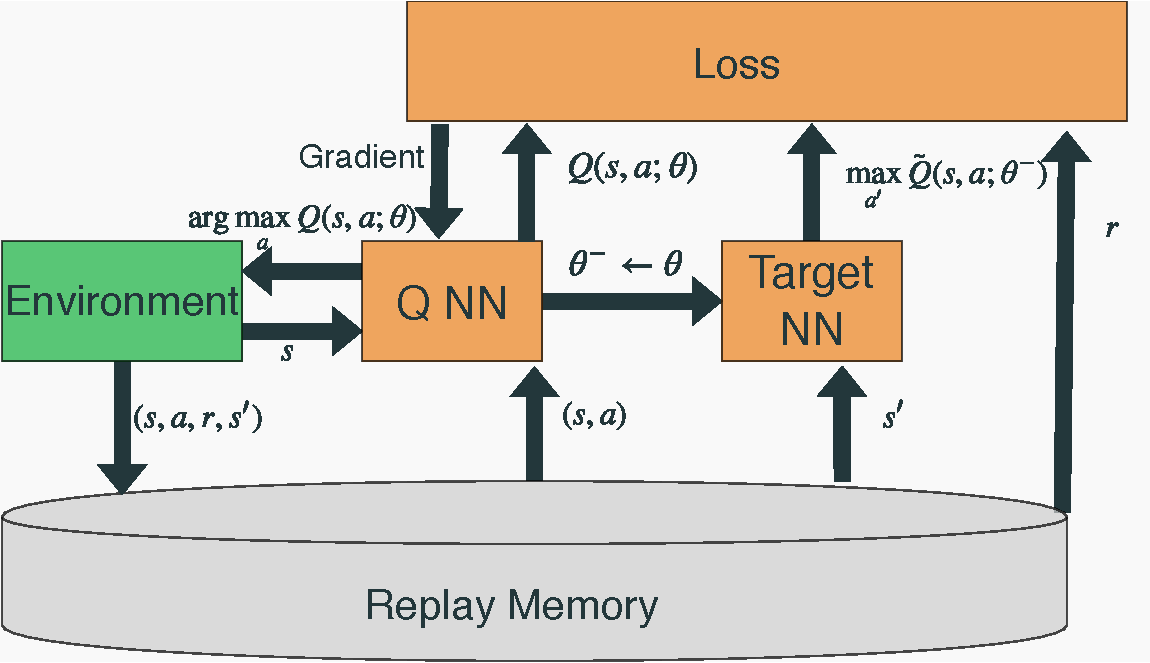
\includegraphics[height=\textheight,width=\textwidth,keepaspectratio]{dqnarchitecture2}
\end{frame}
